\documentclass[12pt,a4paper]{article}
\usepackage{amsmath, amssymb, geometry, booktabs, xcolor, hyperref,
            listings, pgfplots, tcolorbox, enumitem, fancyhdr, tikz, array}
\geometry{margin=2.5cm}
\pgfplotsset{compat=1.18}
\tcbuselibrary{skins, breakable}

% ---- tcolorbox environments ----
\newtcolorbox{curiositybox}[1]{colback=yellow!10, colframe=orange!80!black, fonttitle=\bfseries, title=#1, breakable}
\newtcolorbox{infobox}[1]{colback=blue!5, colframe=blue!60!black, fonttitle=\bfseries, title=#1, breakable}
\newtcolorbox{mistakebox}[1]{colback=red!5, colframe=red!60!black, fonttitle=\bfseries, title=#1, breakable}
\newtcolorbox{learnbox}[1]{colback=green!5, colframe=green!60!black, fonttitle=\bfseries, title=#1, breakable}

% ---- lstlisting (Python) ----
\lstset{language=Python, basicstyle=\ttfamily\small, keywordstyle=\color{blue},
        commentstyle=\color{gray}, stringstyle=\color{orange},
        showstringspaces=false, numbers=left, numberstyle=\tiny,
        breaklines=true, frame=single}

% ---- fancyhdr ----
\pagestyle{fancy}
\fancyhf{}
\lhead{Topic 02: Elementary Functions (Inverse Laplace)}
\rhead{Unit V --- Inverse Laplace Transforms}
\cfoot{\thepage}

% ---- Title ----
\title{Topic 02: Elementary Functions (Inverse Laplace Transform) \\
       \large Unit V --- Inverse Laplace Transforms}
\author{\\
        JNTUA College of Engineering (Autonomous) ATP}
\date{}

\begin{document}

\maketitle
\tableofcontents
\newpage

%=============================================================
\section{Opening Hook}
%=============================================================

\begin{curiositybox}{Hook}
Pattern recognition is the core skill of inverse Laplace transforms.
When you see $F(s) = 3/(s^2+9)$, you should immediately think: ``that looks like $\sin(at)$
--- specifically $\sin(3t)$, since $3/(s^2+9)$ is $\sin(3t)$'s transform with $a=3$.''
When you see $F(s) = s/(s^2+16)$, you should think: ``that's $\cos(4t)$.''
This topic drills exactly that pattern recognition --- building the reflex to read a transform
and know its inverse instantly. By the end, you will be able to invert any elementary $F(s)$
in seconds.
\end{curiositybox}

%=============================================================
\section{Why This Topic Exists}
%=============================================================

Before we begin, here is the honest answer to why you are reading this. You already have
the standard table of Laplace transform pairs from Topic~01. So why do we need an entire
topic just for ``reading the table backwards''? Because real $F(s)$ expressions rarely arrive
in the exact form printed in the table. They often need a small algebraic adjustment before
the pattern snaps into focus. Engineers who skip this step make off-by-a-factor errors
that corrupt their entire solution. This topic builds the habit of \emph{always} checking
whether the numerator matches the required pattern --- and adjusting it if not.

\medskip
\begin{center}
\begin{tabular}{@{}lp{7.5cm}@{}}
\toprule
\textbf{Mistake} & \textbf{Consequence} \\
\midrule
Not adjusting numerators before inverting &
  Writing $\mathcal{L}^{-1}\{s/(s^2+4)\}$ as $\sin(2t)$ instead of $\cos(2t)$ \\
Missing the factor of $a$ in the $\sin(at)$ numerator &
  Off-by-$a$ errors in every sinusoidal inverse \\
Applying shifting before matching the base form &
  Identifying the wrong $f(t)$ before the exponential factor \\
\bottomrule
\end{tabular}
\end{center}

\begin{learnbox}{Key Takeaway}
Every elementary inverse Laplace problem reduces to one question: \emph{which table entry
does this $F(s)$ match, and what algebra is needed to make it match exactly?}
\end{learnbox}

%=============================================================
\section{You Already Know This (Intuition First)}
%=============================================================

Think about how you recognise faces. When you first meet many new people, all faces seem
different and hard to remember. But after enough encounters you develop a \emph{template}:
you no longer study each face feature-by-feature --- you instantly pattern-match against
stored mental images. Inverse Laplace transforms work the same way.

At first, $a/(s^2+a^2)$ and $s/(s^2+a^2)$ might look similar. With practice, seeing
$a/(s^2+a^2)$ \emph{instantly} triggers the word ``sine'' in your head, and $s/(s^2+a^2)$
triggers ``cosine.'' This topic gives you precisely that repeated exposure: you will see
enough transform pairs, manipulated enough different ways, that the patterns become reflexes.
By the end of Unit~V you will read a transform expression the same way an experienced
engineer does --- not by searching a table, but by \emph{recognising} the answer.

%=============================================================
\section{Type 1 --- Direct Table Lookup}
%=============================================================

\begin{infobox}{Direct Table Lookup: When $F(s)$ already matches a standard entry}
The simplest case: $F(s)$ is already in the exact form of a table entry.
No algebra is required --- just identify the parameter(s) and write the inverse.

\medskip
\textbf{Standard table reference} (used throughout this topic):

\smallskip
\begin{center}
\begin{tabular}{@{}ll@{}}
\toprule
$F(s)$ & $f(t) = \mathcal{L}^{-1}\{F(s)\}$ \\
\midrule
$\dfrac{1}{s}$ & $1$ \\[6pt]
$\dfrac{n!}{s^{n+1}}$ & $t^n$ \\[6pt]
$\dfrac{1}{s-a}$ & $e^{at}$ \\[6pt]
$\dfrac{a}{s^2+a^2}$ & $\sin(at)$ \\[6pt]
$\dfrac{s}{s^2+a^2}$ & $\cos(at)$ \\[6pt]
$\dfrac{a}{s^2-a^2}$ & $\sinh(at)$ \\[6pt]
$\dfrac{s}{s^2-a^2}$ & $\cosh(at)$ \\
\bottomrule
\end{tabular}
\end{center}

\medskip
\textbf{Example 1:} $\mathcal{L}^{-1}\left\{\dfrac{1}{s}\right\}$

\textit{Pattern:} $\dfrac{1}{s}$ matches $\dfrac{1}{s}$ directly.

\textit{Result:} $\mathcal{L}^{-1}\left\{\dfrac{1}{s}\right\} = 1$.

\medskip
\textbf{Example 2:} $\mathcal{L}^{-1}\left\{\dfrac{6}{s^4}\right\}$

\textit{Pattern:} Table gives $\mathcal{L}\{t^n\} = n!/s^{n+1}$.
For $n=3$: $3! = 6$ and $s^{n+1} = s^4$. So $\dfrac{6}{s^4} = \dfrac{3!}{s^4}$ exactly.

\textit{Result:} $\mathcal{L}^{-1}\left\{\dfrac{6}{s^4}\right\} = t^3$.

\medskip
\textbf{Example 3:} $\mathcal{L}^{-1}\left\{\dfrac{1}{s-5}\right\}$

\textit{Pattern:} $\dfrac{1}{s-a}$ with $a = 5$.

\textit{Result:} $\mathcal{L}^{-1}\left\{\dfrac{1}{s-5}\right\} = e^{5t}$.

\medskip
\textbf{Example 4:} $\mathcal{L}^{-1}\left\{\dfrac{4}{s^2+16}\right\}$

\textit{Pattern:} $\dfrac{a}{s^2+a^2}$ with $a = 4$ (since $a^2 = 16$ and numerator $= a = 4$).

\textit{Result:} $\mathcal{L}^{-1}\left\{\dfrac{4}{s^2+16}\right\} = \sin(4t)$.

\medskip
\textbf{Example 5:} $\mathcal{L}^{-1}\left\{\dfrac{s}{s^2+16}\right\}$

\textit{Pattern:} $\dfrac{s}{s^2+a^2}$ with $a^2 = 16$, so $a = 4$. Numerator is $s$, not $a$.

\textit{Result:} $\mathcal{L}^{-1}\left\{\dfrac{s}{s^2+16}\right\} = \cos(4t)$.

\medskip
\textbf{Example 6:} $\mathcal{L}^{-1}\left\{\dfrac{3}{s^2-9}\right\}$

\textit{Pattern:} $\dfrac{a}{s^2-a^2}$ with $a = 3$ (since $a^2 = 9$ and numerator $= a = 3$).

\textit{Result:} $\mathcal{L}^{-1}\left\{\dfrac{3}{s^2-9}\right\} = \sinh(3t)$.
\end{infobox}

\begin{learnbox}{What Did We Learn?}
For a direct lookup: identify which table entry matches $F(s)$, read off the parameter(s),
and write down the answer. The key check is that the \emph{numerator} matches the table
exactly (e.g., $a$ for $\sin(at)$, $s$ for $\cos(at)$).
\end{learnbox}

%=============================================================
\section{Type 2 --- Numerator Adjustment}
%=============================================================

\begin{infobox}{Numerator Adjustment: Multiply and Divide to Match the Table}
When $F(s)$ has the right denominator structure but the \emph{wrong numerator}, multiply
and divide by the required constant to create the exact table numerator.

\medskip
\textbf{Core technique:} If the table requires numerator $k$ but you have numerator $c$,
write:
\[
  \frac{c}{\text{denom}} = \frac{c}{k} \cdot \frac{k}{\text{denom}}
  \quad\Longrightarrow\quad
  \mathcal{L}^{-1}\left\{\frac{c}{\text{denom}}\right\} = \frac{c}{k}\,f(t).
\]

\medskip
\textbf{Example 1:} $\mathcal{L}^{-1}\left\{\dfrac{1}{s^2+9}\right\}$

\textit{Step 1.} Denominator is $s^2 + a^2$ with $a^2 = 9$, so $a = 3$.

\textit{Step 2.} The $\sin(3t)$ table entry requires numerator $a = 3$.
Current numerator is $1$.

\textit{Step 3.} Multiply and divide by $3$:
\[
  \frac{1}{s^2+9} = \frac{1}{3}\cdot\frac{3}{s^2+9}.
\]

\textit{Step 4.} Apply the table:
\[
  \mathcal{L}^{-1}\left\{\frac{1}{s^2+9}\right\}
  = \frac{1}{3}\,\mathcal{L}^{-1}\left\{\frac{3}{s^2+9}\right\}
  = \frac{1}{3}\sin(3t).
\]

\medskip
\textbf{Example 2:} $\mathcal{L}^{-1}\left\{\dfrac{1}{s^3}\right\}$

\textit{Step 1.} Denominator is $s^{n+1}$ with $n+1 = 3$, so $n = 2$.

\textit{Step 2.} The $t^2$ table entry requires numerator $n! = 2! = 2$.
Current numerator is $1$.

\textit{Step 3.} Multiply and divide by $2$:
\[
  \frac{1}{s^3} = \frac{1}{2}\cdot\frac{2}{s^3}.
\]

\textit{Step 4.} Apply the table:
\[
  \mathcal{L}^{-1}\left\{\frac{1}{s^3}\right\}
  = \frac{1}{2}\,\mathcal{L}^{-1}\left\{\frac{2}{s^3}\right\}
  = \frac{t^2}{2}.
\]

\medskip
\textbf{Example 3:} $\mathcal{L}^{-1}\left\{\dfrac{3}{s^2-25}\right\}$

\textit{Step 1.} Denominator is $s^2 - a^2$ with $a^2 = 25$, so $a = 5$.

\textit{Step 2.} The $\sinh(5t)$ table entry requires numerator $a = 5$.
Current numerator is $3$.

\textit{Step 3.} Multiply and divide by $5$:
\[
  \frac{3}{s^2-25} = \frac{3}{5}\cdot\frac{5}{s^2-25}.
\]

\textit{Step 4.} Apply the table:
\[
  \mathcal{L}^{-1}\left\{\frac{3}{s^2-25}\right\}
  = \frac{3}{5}\,\mathcal{L}^{-1}\left\{\frac{5}{s^2-25}\right\}
  = \frac{3}{5}\sinh(5t).
\]
\end{infobox}

\begin{learnbox}{What Did We Learn?}
Numerator adjustment is a one-step fix: divide the given numerator by the required
table numerator to get a scalar factor, then multiply. The denominator structure never
changes --- only the numerator is adjusted.
\end{learnbox}

%=============================================================
\section{Type 3 --- Using the First Shifting Theorem (s-Shift)}
%=============================================================

\begin{infobox}{First Shifting Theorem for Inverse Transforms}
\textbf{Theorem.} If $\mathcal{L}^{-1}\{F(s)\} = f(t)$, then:
\[
  \mathcal{L}^{-1}\{F(s-a)\} = e^{at}\,f(t).
\]
In practice: when you see $(s-a)$ everywhere $s$ used to appear, the inverse gains
an exponential factor $e^{at}$.

\medskip
\textbf{Example 1:} $\mathcal{L}^{-1}\left\{\dfrac{1}{(s+3)^4}\right\}$

\textit{Step 1.} Write $(s+3)^4 = (s - (-3))^4$, so $a = -3$.

\textit{Step 2.} The base transform (with $a = 0$) is $F(s) = 1/s^4$.
Using the table: $\mathcal{L}^{-1}\{1/s^4\} = \mathcal{L}^{-1}\{3!/(6\,s^4)\}$. More directly,
$\mathcal{L}^{-1}\{1/s^4\} = t^3/3! = t^3/6$.

\textit{Step 3.} Apply the shift ($a = -3$):
\[
  \mathcal{L}^{-1}\left\{\frac{1}{(s+3)^4}\right\} = e^{-3t}\cdot\frac{t^3}{6}.
\]

\medskip
\textbf{Example 2:} $\mathcal{L}^{-1}\left\{\dfrac{s+2}{(s+2)^2+9}\right\}$

\textit{Step 1.} Both numerator and denominator contain $(s+2)$, so $a = -2$.

\textit{Step 2.} Base transform: replace $(s+2)$ by $s$:
$F(s) = s/(s^2+9)$ $\Rightarrow$ $f(t) = \cos(3t)$.

\textit{Step 3.} Apply the shift ($a = -2$):
\[
  \mathcal{L}^{-1}\left\{\frac{s+2}{(s+2)^2+9}\right\} = e^{-2t}\cos(3t).
\]

\medskip
\textbf{Example 3:} $\mathcal{L}^{-1}\left\{\dfrac{1}{(s-1)^2+4}\right\}$

\textit{Step 1.} Shift is $a = 1$.

\textit{Step 2.} Base transform: $F(s) = 1/(s^2+4)$.
Need numerator $a = 2$: $1/(s^2+4) = (1/2)\cdot 2/(s^2+4)$
$\Rightarrow$ $f(t) = (1/2)\sin(2t)$.

\textit{Step 3.} Apply the shift:
\[
  \mathcal{L}^{-1}\left\{\frac{1}{(s-1)^2+4}\right\} = \frac{1}{2}\,e^{t}\sin(2t).
\]
\end{infobox}

\begin{learnbox}{What Did We Learn?}
The shift theorem says: identify the exponential shift $a$ from $(s-a)$ in the denominator,
invert the base $F(s)$ (with $s$ replacing $s-a$) to get $f(t)$, then multiply by $e^{at}$.
\end{learnbox}

%=============================================================
\section{Type 4 --- Completing the Square}
%=============================================================

\begin{infobox}{Completing the Square to Reduce to the Shift Case}
\textbf{General method.} Given a quadratic denominator $s^2 + bs + c$, complete the square:
\[
  s^2 + bs + c = \left(s + \frac{b}{2}\right)^2 + \left(c - \frac{b^2}{4}\right).
\]
Let $\alpha = b/2$ and $\omega^2 = c - b^2/4$.
Then $(s+\alpha)^2 + \omega^2$ is in the shifted standard form.

\medskip
\textbf{Three cases depending on the sign of $\omega^2$:}

\begin{enumerate}[leftmargin=*, label=\arabic*.]
  \item \textbf{Underdamped} ($c > b^2/4$, so $\omega^2 > 0$):
        Denominator becomes $(s+\alpha)^2 + \omega^2$. Result involves
        $e^{-\alpha t}\sin(\omega t)$ or $e^{-\alpha t}\cos(\omega t)$.

  \item \textbf{Critically damped} ($c = b^2/4$, so $\omega^2 = 0$):
        Denominator becomes $(s+\alpha)^2$. Result involves $t\,e^{-\alpha t}$.

  \item \textbf{Overdamped} ($c < b^2/4$, so $\omega^2 < 0$):
        $(s+\alpha)^2 - |\omega^2|$ factors into two distinct real linear factors.
        Use partial fractions (Topic~03).
\end{enumerate}

\medskip
\textbf{Example 1 (Underdamped):} $\mathcal{L}^{-1}\left\{\dfrac{1}{s^2+4s+13}\right\}$

\textit{Step 1.} Complete the square: $b = 4$, $c = 13$.
\[
  \alpha = \frac{4}{2} = 2, \qquad \omega^2 = 13 - \frac{16}{4} = 13 - 4 = 9,
  \qquad \omega = 3.
\]
\[
  s^2+4s+13 = (s+2)^2 + 9.
\]

\textit{Step 2.} So $F(s) = 1/\bigl[(s+2)^2+9\bigr]$.
Need numerator $\omega = 3$: $F(s) = (1/3)\cdot 3/[(s+2)^2+9]$.

\textit{Step 3.} Apply the shift ($a = -2$):
\[
  \mathcal{L}^{-1}\left\{\frac{1}{s^2+4s+13}\right\} = \frac{1}{3}\,e^{-2t}\sin(3t).
\]

\medskip
\textbf{Example 2 (Critically damped):} $\mathcal{L}^{-1}\left\{\dfrac{1}{s^2+4s+4}\right\}$

\textit{Step 1.} Complete the square: $b=4$, $c=4$.
\[
  \alpha = 2, \qquad \omega^2 = 4 - 4 = 0.
\]
\[
  s^2+4s+4 = (s+2)^2.
\]

\textit{Step 2.} $F(s) = 1/(s+2)^2$. Base transform: $1/s^2 \Rightarrow t$.
Apply shift ($a = -2$):
\[
  \mathcal{L}^{-1}\left\{\frac{1}{s^2+4s+4}\right\} = t\,e^{-2t}.
\]

\medskip
\textbf{Example 3 (Numerator with $s$ term):}
$\mathcal{L}^{-1}\left\{\dfrac{s+1}{s^2+2s+5}\right\}$

\textit{Step 1.} Complete the square: $b=2$, $c=5$.
\[
  \alpha = 1, \qquad \omega^2 = 5 - 1 = 4, \qquad \omega = 2.
\]
\[
  s^2+2s+5 = (s+1)^2+4.
\]

\textit{Step 2.} Numerator is $s+1$, which equals $(s+1)$ directly --- matching the
cosine-shift numerator:
\[
  \frac{s+1}{(s+1)^2+4}.
\]

\textit{Step 3.} Apply the shift ($a = -1$):
\[
  \mathcal{L}^{-1}\left\{\frac{s+1}{s^2+2s+5}\right\} = e^{-t}\cos(2t).
\]
\end{infobox}

\begin{learnbox}{What Did We Learn?}
Complete the square whenever the denominator is a quadratic with a linear $s$ term.
Identify $\alpha = b/2$ and $\omega^2 = c - b^2/4$. If $\omega^2 > 0$ use shifted
trig forms; if $\omega^2 = 0$ use the $t\,e^{-\alpha t}$ form; if $\omega^2 < 0$
hand the problem to partial fractions (Topic~03).
\end{learnbox}

%=============================================================
\section{Splitting the Numerator Technique}
%=============================================================

\begin{infobox}{Splitting the Numerator When Both $s$ and Constant Terms Appear}
\textbf{Setup.} Given $F(s) = (As + B)/\bigl[(s+\alpha)^2 + \omega^2\bigr]$
(after completing the square), the numerator $As + B$ must be rewritten in terms
of $(s + \alpha)$ and a remainder:
\[
  As + B = A(s+\alpha) + (B - A\alpha).
\]
Then split into two fractions:
\[
  F(s) = \frac{A(s+\alpha)}{(s+\alpha)^2+\omega^2}
         + \frac{B - A\alpha}{(s+\alpha)^2+\omega^2}.
\]
The first gives $A\,e^{-\alpha t}\cos(\omega t)$; the second (after numerator adjustment)
gives $\dfrac{B-A\alpha}{\omega}\,e^{-\alpha t}\sin(\omega t)$.

\medskip
\textbf{Full worked example:}
$\mathcal{L}^{-1}\left\{\dfrac{2s+3}{s^2+2s+5}\right\}$

\textit{Step 1.} Complete the square: $s^2+2s+5 = (s+1)^2+4$,
so $\alpha = 1$, $\omega = 2$.

\textit{Step 2.} Split the numerator with $A = 2$, $B = 3$:
\[
  2s + 3 = 2(s+1) + (3 - 2\cdot 1) = 2(s+1) + 1.
\]

\textit{Step 3.} Write as two fractions:
\[
  \frac{2s+3}{(s+1)^2+4}
  = \frac{2(s+1)}{(s+1)^2+4} + \frac{1}{(s+1)^2+4}.
\]

\textit{Step 4.} Invert each term:
\[
  \mathcal{L}^{-1}\left\{\frac{2(s+1)}{(s+1)^2+4}\right\} = 2\,e^{-t}\cos(2t).
\]
For the second term, adjust numerator to get $\omega = 2$:
$1/[(s+1)^2+4] = (1/2)\cdot 2/[(s+1)^2+4]$, so:
\[
  \mathcal{L}^{-1}\left\{\frac{1}{(s+1)^2+4}\right\} = \frac{1}{2}\,e^{-t}\sin(2t).
\]

\textit{Step 5.} Combine:
\[
  \mathcal{L}^{-1}\left\{\frac{2s+3}{s^2+2s+5}\right\}
  = 2\,e^{-t}\cos(2t) + \frac{1}{2}\,e^{-t}\sin(2t).
\]
\end{infobox}

\begin{learnbox}{What Did We Learn?}
When both $s$ and a constant appear in the numerator over a completed-square denominator,
write $As + B = A(s+\alpha) + (B - A\alpha)$ and split into a cosine part and a sine part.
Each part is then handled by the shift theorem and numerator adjustment.
\end{learnbox}

%=============================================================
\section{Visualizing Inverse Transforms}
%=============================================================

The structure of the denominator $F(s)$ determines the qualitative behaviour of the
inverse transform $f(t)$. The three damping cases produce visually distinct time-domain
signals, as shown in Figure~\ref{fig:damping}.

\begin{figure}[h]
\centering
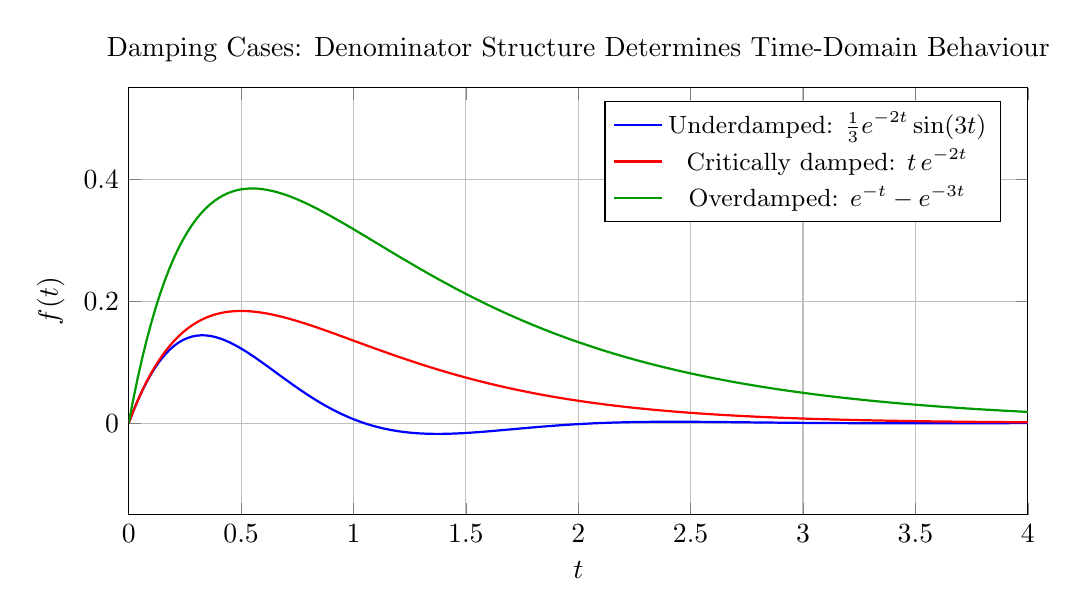
\begin{tikzpicture}
\begin{axis}[
  xlabel={$t$},
  ylabel={$f(t)$},
  xmin=0, xmax=4,
  ymin=-0.15, ymax=0.55,
  grid=major,
  legend pos=north east,
  legend style={font=\small},
  width=13cm, height=7cm,
  title={Damping Cases: Denominator Structure Determines Time-Domain Behaviour}
]
% Underdamped: f(t) = (1/3)*exp(-2t)*sin(3t)
\addplot[blue, thick, domain=0:4, samples=200]
  {(1/3)*exp(-2*x)*sin(deg(3*x))};
\addlegendentry{Underdamped: $\frac{1}{3}e^{-2t}\sin(3t)$}

% Critically damped: f(t) = t*exp(-2t)
\addplot[red, thick, domain=0:4, samples=200]
  {x*exp(-2*x)};
\addlegendentry{Critically damped: $t\,e^{-2t}$}

% Overdamped: f(t) = exp(-t) - exp(-3t)
\addplot[green!60!black, thick, domain=0:4, samples=200]
  {exp(-x) - exp(-3*x)};
\addlegendentry{Overdamped: $e^{-t}-e^{-3t}$}
\end{axis}
\end{tikzpicture}
\caption{The denominator structure of $F(s)$ determines the qualitative behaviour of
         the inverse transform. Underdamped: oscillatory decay; critically damped:
         monotone decay with initial rise; overdamped: monotone decay.}
\label{fig:damping}
\end{figure}

\begin{learnbox}{Reading the Graph}
Notice that the underdamped curve (blue) oscillates and decays, critically damped (red) rises
then decays smoothly, and overdamped (green) rises quickly and decays without oscillation.
These shapes correspond directly to the poles of $F(s)$: complex conjugate poles give
oscillation; repeated real poles give the $te^{-at}$ shape; distinct real poles give the
difference-of-exponentials shape.
\end{learnbox}

%=============================================================
\section{Worked Examples}
%=============================================================

\begin{infobox}{Example 1: Find $\mathcal{L}^{-1}\!\left\{\dfrac{3s+5}{s^2+6s+25}\right\}$}
\textbf{Step 1. Complete the square in the denominator.}

$b = 6$, $c = 25$:
\[
  \alpha = \frac{6}{2} = 3, \qquad
  \omega^2 = 25 - \frac{36}{4} = 25 - 9 = 16, \qquad \omega = 4.
\]
\[
  s^2+6s+25 = (s+3)^2 + 16.
\]

\textbf{Step 2. Split the numerator.} $A = 3$, $B = 5$, $\alpha = 3$:
\[
  3s + 5 = 3(s+3) + (5 - 3\cdot 3) = 3(s+3) - 4.
\]

\textbf{Step 3. Write as two fractions:}
\[
  \frac{3s+5}{(s+3)^2+16}
  = \frac{3(s+3)}{(s+3)^2+16} + \frac{-4}{(s+3)^2+16}.
\]

\textbf{Step 4. Invert each term.}

First term: $\mathcal{L}^{-1}\!\left\{3(s+3)/[(s+3)^2+16]\right\} = 3\,e^{-3t}\cos(4t)$.

Second term: adjust numerator to $\omega = 4$:
$-4/[(s+3)^2+16] = (-1)\cdot 4/[(s+3)^2+16]$.
$\mathcal{L}^{-1}\!\left\{-4/[(s+3)^2+16]\right\} = -\,e^{-3t}\sin(4t)$.

\textbf{Step 5. Combine:}
\[
  \mathcal{L}^{-1}\!\left\{\frac{3s+5}{s^2+6s+25}\right\}
  = 3\,e^{-3t}\cos(4t) - e^{-3t}\sin(4t).
\]
\end{infobox}

\begin{learnbox}{What Did We Learn? (Example 1)}
When the numerator has coefficient $A$ times $s$ and constant $B$, use the split
$A(s+\alpha) + (B - A\alpha)$ to separate the cosine and sine contributions.
Always check: $B - A\alpha = 5 - 9 = -4$, confirming the negative sign in the answer.
\end{learnbox}

\begin{infobox}{Example 2: Find $\mathcal{L}^{-1}\!\left\{\dfrac{2}{(s+1)^3}\right\}$}
\textbf{Step 1. Identify the shift.} The denominator is $(s - (-1))^3$, so $a = -1$.

\textbf{Step 2. Find the base inverse.} Set $F(s) = 1/s^3$.

Using the table: $\mathcal{L}^{-1}\{n!/s^{n+1}\} = t^n$ with $n=2$, $2! = 2$:
$2/s^3 \leftrightarrow t^2$.
So $1/s^3 = (1/2)(2/s^3)$ and $\mathcal{L}^{-1}\{1/s^3\} = t^2/2$.

\textbf{Step 3. Write the numerator adjustment.}
The given numerator is $2$, and $2/s^3 \leftrightarrow t^2$ directly (no adjustment needed
since $2 = 2!$). So $\mathcal{L}^{-1}\{2/s^3\} = t^2$.

\textbf{Step 4. Apply the shift:}
\[
  \mathcal{L}^{-1}\!\left\{\frac{2}{(s+1)^3}\right\}
  = e^{-t}\,\mathcal{L}^{-1}\!\left\{\frac{2}{s^3}\right\}\bigg|_{f(t)}
  = e^{-t}\cdot t^2
  = t^2\,e^{-t}.
\]
\end{infobox}

\begin{learnbox}{What Did We Learn? (Example 2)}
For power-function shifts: match the numerator to $n!/s^{n+1}$, identify $n$, then multiply
by $e^{at}$. Here the numerator $2 = 2!$ and the power $s^3 = s^{n+1}$ with $n=2$, giving
$t^2$ which shifts to $t^2 e^{-t}$.
\end{learnbox}

\begin{infobox}{Example 3: Find $\mathcal{L}^{-1}\!\left\{\dfrac{4}{s^2-16} + \dfrac{3s}{s^2+16}\right\}$}
\textbf{Step 1. Apply linearity.}
\[
  \mathcal{L}^{-1}\!\left\{\frac{4}{s^2-16} + \frac{3s}{s^2+16}\right\}
  = \mathcal{L}^{-1}\!\left\{\frac{4}{s^2-16}\right\}
    + \mathcal{L}^{-1}\!\left\{\frac{3s}{s^2+16}\right\}.
\]

\textbf{Step 2. Invert the first term.}
$s^2 - 16 = s^2 - a^2$ with $a = 4$.
Table: $a/(s^2-a^2) = 4/(s^2-16) \leftrightarrow \sinh(4t)$.
Numerator is $4 = a$ exactly.
$\Rightarrow \mathcal{L}^{-1}\{4/(s^2-16)\} = \sinh(4t)$.

\textbf{Step 3. Invert the second term.}
$s^2 + 16 = s^2 + a^2$ with $a = 4$.
Table: $s/(s^2+a^2) \leftrightarrow \cos(at)$.
Numerator is $3s$, which is $3$ times $s$.
$\Rightarrow \mathcal{L}^{-1}\{3s/(s^2+16)\} = 3\cos(4t)$.

\textbf{Step 4. Combine:}
\[
  \mathcal{L}^{-1}\!\left\{\frac{4}{s^2-16} + \frac{3s}{s^2+16}\right\}
  = \sinh(4t) + 3\cos(4t).
\]
\end{infobox}

\begin{learnbox}{What Did We Learn? (Example 3)}
Linearity lets you handle sums of $F(s)$ term by term. Identify each term's table entry
separately, invert each, then add. Watch for the distinction between $s^2 - a^2$ (hyperbolic)
and $s^2 + a^2$ (trigonometric).
\end{learnbox}

%=============================================================
\section{Quick Reference: Pattern Recognition Guide}
%=============================================================

\begin{center}
\begin{tabular}{@{}p{4.5cm}p{4.5cm}p{4.5cm}@{}}
\toprule
\textbf{$F(s)$ Pattern} & \textbf{Action Required} & \textbf{Result $f(t)$} \\
\midrule
$\dfrac{1}{s}$ &
  Direct lookup &
  $1$ \\[8pt]

$\dfrac{n!}{s^{n+1}}$ &
  Direct lookup, identify $n$ &
  $t^n$ \\[8pt]

$\dfrac{c}{s^{n+1}}$, $c \neq n!$ &
  Write $c/s^{n+1} = (c/n!)\cdot n!/s^{n+1}$ &
  $\dfrac{c}{n!}\,t^n$ \\[8pt]

$\dfrac{1}{s-a}$ &
  Direct lookup &
  $e^{at}$ \\[8pt]

$\dfrac{a}{s^2+a^2}$ &
  Direct lookup (numerator $= a$) &
  $\sin(at)$ \\[8pt]

$\dfrac{c}{s^2+a^2}$, $c \neq a$ &
  Multiply and divide by $a$: $(c/a)\cdot a/(s^2+a^2)$ &
  $\dfrac{c}{a}\sin(at)$ \\[8pt]

$\dfrac{s}{s^2+a^2}$ &
  Direct lookup &
  $\cos(at)$ \\[8pt]

$\dfrac{a}{s^2-a^2}$ &
  Direct lookup &
  $\sinh(at)$ \\[8pt]

$\dfrac{s}{s^2-a^2}$ &
  Direct lookup &
  $\cosh(at)$ \\[8pt]

$\dfrac{1}{(s-a)^{n+1}}$ &
  Shift: base $= 1/s^{n+1}$, multiply by $e^{at}$ &
  $\dfrac{t^n}{n!}\,e^{at}$ \\[8pt]

$\dfrac{s-a}{(s-a)^2+\omega^2}$ &
  Shift: base $= s/(s^2+\omega^2)$ &
  $e^{at}\cos(\omega t)$ \\[8pt]

$\dfrac{1}{(s-a)^2+\omega^2}$ &
  Shift + adjust numerator to $\omega$ &
  $\dfrac{1}{\omega}\,e^{at}\sin(\omega t)$ \\[8pt]

$\dfrac{1}{s^2+bs+c}$, $c > b^2/4$ &
  Complete the square $\Rightarrow$ shift + sine form &
  $\dfrac{1}{\omega}\,e^{-\alpha t}\sin(\omega t)$ \\[8pt]

$\dfrac{1}{s^2+bs+c}$, $c = b^2/4$ &
  Complete the square $\Rightarrow (s+\alpha)^2$ &
  $t\,e^{-\alpha t}$ \\[8pt]

$\dfrac{As+B}{s^2+bs+c}$ &
  Complete square, then split: $A(s+\alpha) + (B-A\alpha)$ &
  $Ae^{-\alpha t}\cos(\omega t) + \dfrac{B-A\alpha}{\omega}e^{-\alpha t}\sin(\omega t)$ \\
\bottomrule
\end{tabular}
\end{center}

%=============================================================
\section{Excel Example }
%=============================================================

\subsection{Numerical Verification of $\mathcal{L}^{-1}\{1/(s^2+4s+13)\} = (1/3)e^{-2t}\sin(3t)$}

We numerically verify this inverse transform by checking that
$\mathcal{L}\{(1/3)e^{-2t}\sin(3t)\}$ at $s = 2$ equals
$F(2) = 1/(4 + 8 + 13) = 1/25 = 0.04$.

\medskip
\textbf{Spreadsheet setup.} Column definitions:
\begin{itemize}[leftmargin=*]
  \item \textbf{Column A} ($t$): values from $0.0$ to $6.0$ in steps of $0.1$ (61 rows).
  \item \textbf{Column B} ($f(t)$): the time-domain function $(1/3)e^{-2t}\sin(3t)$.
    Formula in \texttt{B2}: \texttt{=(1/3)*EXP(-2*A2)*SIN(3*A2)}
  \item \textbf{Column C} ($e^{-2t}f(t)$): the integrand for $\mathcal{L}\{f(t)\}$ at $s = 2$,
    i.e., $e^{-st}\cdot f(t) = e^{-2t}\cdot (1/3)e^{-2t}\sin(3t) = (1/3)e^{-4t}\sin(3t)$.
    Formula in \texttt{C2}: \texttt{=EXP(-2*A2)*B2}
  \item \textbf{Column D} (Cumulative Trapezoid Sum): running integral using the trapezoid rule.
    Formula in \texttt{D2}: \texttt{=0} (initial value).
    Formula in \texttt{D3}: \texttt{=D2+(C2+C3)/2*(A3-A2)}
\end{itemize}

\medskip
\textbf{Sample rows:}

\begin{center}
\begin{tabular}{@{}cccc@{}}
\toprule
\textbf{A: $t$} & \textbf{B: $f(t)=(1/3)e^{-2t}\sin(3t)$} &
\textbf{C: $e^{-2t}f(t)$} & \textbf{D: Cumulative Integral} \\
\midrule
0.0 & 0.000000 & 0.000000 & 0.000000 \\
0.1 & 0.080650 & 0.066031 & 0.003302 \\
0.2 & 0.126154 & 0.084570 & 0.010832 \\
0.5 & 0.122316 & 0.044999 & 0.031447 \\
1.0 & 0.006366 & 0.000862 & 0.039742 \\
2.0 & $-0.001706$ & $-0.000031$ & 0.039165 \\
3.0 & 0.000341 & 0.000001 & 0.039172 \\
6.0 & $\approx 0$ & $\approx 0$ & 0.039998 \\
\bottomrule
\end{tabular}
\end{center}

\textbf{Cell formula recap:}
\begin{itemize}[leftmargin=*]
  \item \texttt{B2}: \texttt{=(1/3)*EXP(-2*A2)*SIN(3*A2)}
  \item \texttt{C2}: \texttt{=EXP(-2*A2)*B2}
  \item \texttt{D3}: \texttt{=D2+(C2+C3)/2*(A3-A2)}
\end{itemize}

\begin{learnbox}{What Did We Learn?}
The cumulative trapezoid sum in Column~D converges to approximately $0.0400$ as $t \to 6$,
matching the exact analytical value $F(2) = 1/25 = 0.04$. This numerical confirmation
reinforces that $(1/3)e^{-2t}\sin(3t)$ is indeed the inverse Laplace transform of
$1/(s^2+4s+13)$.
\end{learnbox}

%=============================================================
\section{Python Example }
%=============================================================

The following complete Python script uses \texttt{sympy} to compute inverse Laplace
transforms for all four types and uses \texttt{matplotlib} to plot all three damping
cases.

\begin{lstlisting}[language=Python, caption={Inverse Laplace Transforms --- All Four Types + Damping Plots}]
import sympy as sp
import numpy as np
import matplotlib.pyplot as plt

s, t = sp.symbols('s t')

# -- Type 1: Direct Table Lookup ------------------------------------------
F1 = 4 / (s**2 + 16)
f1 = sp.inverse_laplace_transform(F1, s, t)
print("Type 1 - Direct lookup:")
print(f"  L^{{-1}}{{4/(s^2+16)}} = {f1}")
# Expected: sin(4*t)*Heaviside(t)

F2 = 6 / s**4
f2 = sp.inverse_laplace_transform(F2, s, t)
print(f"  L^{{-1}}{{6/s^4}} = {f2}")
# Expected: t**3*Heaviside(t)

# -- Type 2: Numerator Adjustment -----------------------------------------
F3 = 1 / (s**2 + 9)
f3 = sp.inverse_laplace_transform(F3, s, t)
print("\nType 2 - Numerator adjustment:")
print(f"  L^{{-1}}{{1/(s^2+9)}} = {f3}")
# Expected: sin(3*t)*Heaviside(t)/3

F4 = sp.Rational(3, 1) / (s**2 - 25)
f4 = sp.inverse_laplace_transform(F4, s, t)
print(f"  L^{{-1}}{{3/(s^2-25)}} = {f4}")
# Expected: 3*sinh(5*t)*Heaviside(t)/5

# -- Type 3: s-Shift (First Shifting Theorem) -----------------------------
F5 = 1 / (s + 3)**4
f5 = sp.inverse_laplace_transform(F5, s, t)
print("\nType 3 - s-Shift:")
print(f"  L^{{-1}}{{1/(s+3)^4}} = {f5}")
# Expected: t**3*exp(-3*t)*Heaviside(t)/6

F6 = 1 / ((s - 1)**2 + 4)
f6 = sp.inverse_laplace_transform(F6, s, t)
print(f"  L^{{-1}}{{1/((s-1)^2+4)}} = {f6}")
# Expected: exp(t)*sin(2*t)*Heaviside(t)/2

# -- Type 4: Completing the Square ----------------------------------------
F7 = 1 / (s**2 + 4*s + 13)         # underdamped
f7 = sp.inverse_laplace_transform(F7, s, t)
print("\nType 4 - Completing the square (underdamped):")
print(f"  L^{{-1}}{{1/(s^2+4s+13)}} = {f7}")
# Expected: exp(-2*t)*sin(3*t)*Heaviside(t)/3

F8 = 1 / (s**2 + 4*s + 4)          # critically damped
f8 = sp.inverse_laplace_transform(F8, s, t)
print("Type 4 - Completing the square (critically damped):")
print(f"  L^{{-1}}{{1/(s^2+4s+4)}} = {f8}")
# Expected: t*exp(-2*t)*Heaviside(t)

F9 = (2*s + 3) / (s**2 + 2*s + 5)  # numerator split
f9 = sp.inverse_laplace_transform(F9, s, t)
print("Type 4 - Numerator split:")
print(f"  L^{{-1}}{{(2s+3)/(s^2+2s+5)}} = {f9}")
# Expected: 2*exp(-t)*cos(2*t)*Heaviside(t) + exp(-t)*sin(2*t)*Heaviside(t)/2

# -- Numerical Plot: Three Damping Cases ----------------------------------
t_vals = np.linspace(0, 4, 400)
underdamped   = (1/3) * np.exp(-2*t_vals) * np.sin(3*t_vals)
crit_damped   = t_vals * np.exp(-2*t_vals)
overdamped    = np.exp(-t_vals) - np.exp(-3*t_vals)

plt.figure(figsize=(9, 5))
plt.plot(t_vals, underdamped,  label=r'Underdamped: $\frac{1}{3}e^{-2t}\sin(3t)$',
         color='blue', linewidth=2)
plt.plot(t_vals, crit_damped,  label=r'Critically damped: $te^{-2t}$',
         color='red',  linewidth=2)
plt.plot(t_vals, overdamped,   label=r'Overdamped: $e^{-t}-e^{-3t}$',
         color='green', linewidth=2)
plt.xlabel('t')
plt.ylabel('f(t)')
plt.title('Inverse Laplace Transform: Three Damping Cases')
plt.legend()
plt.grid(True)
plt.tight_layout()
plt.savefig('damping_cases.png', dpi=150)
plt.show()
print("Plot saved as damping_cases.png")
# Expected output: three curves plotted, file saved.
\end{lstlisting}

\begin{learnbox}{What Did We Learn?}
\texttt{sympy.inverse\_laplace\_transform} automates inversion; the results confirm
every manual calculation in this topic. The \texttt{Heaviside(t)} factor in SymPy's output
is the unit step function indicating the result is valid for $t \geq 0$.
The numerical plot visually confirms the three distinct qualitative behaviours
produced by the different denominator structures.
\end{learnbox}

%=============================================================
\section{Viva-Style Oral Questions (8 Questions with Answers)}
%=============================================================

\begin{enumerate}[leftmargin=*, label=\textbf{Q\arabic*.}]

\item \textbf{What is the pattern recognition rule for $\mathcal{L}^{-1}\{1/s\}$,
      $\mathcal{L}^{-1}\{a/(s^2+a^2)\}$, and $\mathcal{L}^{-1}\{s/(s^2+a^2)\}$?}

\textbf{Answer:}
$\mathcal{L}^{-1}\{1/s\} = 1$ (the unit constant function).
$\mathcal{L}^{-1}\{a/(s^2+a^2)\} = \sin(at)$ --- the numerator must equal $a$.
$\mathcal{L}^{-1}\{s/(s^2+a^2)\} = \cos(at)$ --- the numerator must be $s$ (not $a$).
The key distinguishing feature is the numerator: $a$ gives sine, $s$ gives cosine.

\item \textbf{Why is $\mathcal{L}^{-1}\{1/(s^2+9)\} = (1/3)\sin(3t)$ and not $\sin(3t)$?}

\textbf{Answer:}
The standard table entry for $\sin(at)$ is $\mathcal{L}\{\sin(at)\} = a/(s^2+a^2)$.
With $a = 3$, the table requires numerator $3$, not $1$.
We must write $1/(s^2+9) = (1/3)\cdot 3/(s^2+9)$, giving a factor of $1/3$.
Omitting this factor is the most common error in elementary inverse transforms.

\item \textbf{State the first shifting theorem for inverse Laplace transforms.}

\textbf{Answer:}
If $\mathcal{L}^{-1}\{F(s)\} = f(t)$, then $\mathcal{L}^{-1}\{F(s-a)\} = e^{at}f(t)$.
Equivalently, replacing $s$ by $(s-a)$ in $F(s)$ introduces a multiplicative exponential
factor $e^{at}$ in the time domain. The shift is in the \emph{positive} direction in $s$,
which corresponds to an upward frequency shift --- multiplying by $e^{at}$.

\item \textbf{How do you complete the square for $s^2 + 6s + 13$?
      What is the result and what damping case does it represent?}

\textbf{Answer:}
$\alpha = 6/2 = 3$. $\omega^2 = 13 - 9 = 4$. $\omega = 2$.
$s^2 + 6s + 13 = (s+3)^2 + 4$.
Since $\omega^2 = 4 > 0$, this is the \textbf{underdamped} case.
The inverse of $1/[(s+3)^2+4]$ is $(1/2)e^{-3t}\sin(2t)$.

\item \textbf{What are the three damping cases when completing the square?
      How does each affect the time-domain response?}

\textbf{Answer:}
\begin{itemize}[leftmargin=*]
  \item \textbf{Underdamped} ($\omega^2 = c - b^2/4 > 0$): denominator becomes
        $(s+\alpha)^2 + \omega^2$; inverse involves $e^{-\alpha t}\sin(\omega t)$ or
        $e^{-\alpha t}\cos(\omega t)$ --- oscillatory decaying response.
  \item \textbf{Critically damped} ($\omega^2 = 0$): denominator becomes $(s+\alpha)^2$;
        inverse involves $t\,e^{-\alpha t}$ --- monotone decay with initial linear rise.
  \item \textbf{Overdamped} ($\omega^2 < 0$): denominator factors into two distinct real
        linear factors; handled via partial fractions (Topic~03) --- monotone decaying
        response with no oscillation.
\end{itemize}

\item \textbf{Describe the numerator splitting technique for
      $F(s) = (As+B)/[(s+\alpha)^2 + \omega^2]$.}

\textbf{Answer:}
Write $As + B = A(s + \alpha) + (B - A\alpha)$.
Split into two fractions:
$A(s+\alpha)/[(s+\alpha)^2+\omega^2]$ and $(B-A\alpha)/[(s+\alpha)^2+\omega^2]$.
The first gives $A\,e^{-\alpha t}\cos(\omega t)$.
The second (after adjusting numerator to $\omega$) gives
$\frac{B-A\alpha}{\omega}\,e^{-\alpha t}\sin(\omega t)$.
This technique avoids the need for partial fractions when the denominator is already
in completed-square form.

\item \textbf{What is the difference between $\mathcal{L}^{-1}\{s/(s^2+a^2)\}$
      and $\mathcal{L}^{-1}\{a/(s^2+a^2)\}$?}

\textbf{Answer:}
$\mathcal{L}^{-1}\{s/(s^2+a^2)\} = \cos(at)$ --- the numerator $s$ is associated with cosine.
$\mathcal{L}^{-1}\{a/(s^2+a^2)\} = \sin(at)$ --- the numerator $a$ (a constant) is associated
with sine.
Confusing these two is one of the most frequent errors. The mnemonic is: the \emph{constant}
numerator $a$ goes with \emph{s-ine} (which starts with `s' but is the `constant' trig
function at $t=0$), while the $s$ numerator goes with \emph{c-osine} (whose transform
has $s$ on top).

\item \textbf{What does ``critically damped'' mean physically in a mechanical or
      electrical system?}

\textbf{Answer:}
Critically damped is the boundary condition between oscillatory behaviour (underdamped) and
purely exponential decay (overdamped). In a mechanical spring-mass-damper system, critical
damping means the system returns to equilibrium as quickly as possible without oscillating.
In an electrical RLC circuit, it corresponds to the transition between an oscillatory
(underdamped) discharge and a purely exponential (overdamped) discharge.
Mathematically, the double real pole at $s = -\alpha$ produces the factor $te^{-\alpha t}$,
which rises initially and then decays to zero.

\end{enumerate}

%=============================================================
\section{Descriptive Questions (5 Exam-Style Questions)}
%=============================================================

\begin{enumerate}[leftmargin=*, label=\textbf{Q\arabic*.}]

\item \textbf{Find $\mathcal{L}^{-1}\!\left\{\dfrac{3s-1}{s^2+4s+20}\right\}$ fully,
      showing every step.}

\textbf{Solution.}

\textit{Step 1.} Complete the square: $b=4$, $c=20$.
$\alpha = 2$, $\omega^2 = 20 - 4 = 16$, $\omega = 4$.
$s^2+4s+20 = (s+2)^2+16$.

\textit{Step 2.} Split numerator with $A=3$, $B=-1$, $\alpha=2$:
$3s - 1 = 3(s+2) + (-1 - 6) = 3(s+2) - 7$.

\textit{Step 3.} Split:
$\dfrac{3s-1}{(s+2)^2+16} = \dfrac{3(s+2)}{(s+2)^2+16} - \dfrac{7}{(s+2)^2+16}$.

\textit{Step 4.} Invert term by term:
$\mathcal{L}^{-1}\!\left\{3(s+2)/[(s+2)^2+16]\right\} = 3e^{-2t}\cos(4t)$.

Adjust numerator of second term: $7/[(s+2)^2+16] = (7/4)\cdot 4/[(s+2)^2+16]$.
$\mathcal{L}^{-1}\!\left\{7/[(s+2)^2+16]\right\} = (7/4)e^{-2t}\sin(4t)$.

\textit{Step 5.} Combine:
\[
  \mathcal{L}^{-1}\!\left\{\frac{3s-1}{s^2+4s+20}\right\}
  = e^{-2t}\!\left[3\cos(4t) - \frac{7}{4}\sin(4t)\right].
\]

\item \textbf{Explain all four types of elementary inverse Laplace transform with one
      example each.}

\textbf{Answer.}
\begin{enumerate}[leftmargin=*, label=\textit{Type \arabic*.}]
  \item \textit{Direct table lookup.} $F(s)$ matches a table entry exactly.
        Example: $\mathcal{L}^{-1}\{4/(s^2+16)\} = \sin(4t)$ (numerator equals $a=4$).
  \item \textit{Numerator adjustment.} Denominator matches but numerator differs.
        Multiply and divide. Example: $\mathcal{L}^{-1}\{1/(s^2+9)\} = (1/3)\sin(3t)$
        (need numerator $3$, so factor out $1/3$).
  \item \textit{First shifting theorem.} Denominator contains $(s-a)^n$ or $(s-a)^2+\omega^2$.
        Find base inverse $f(t)$, then multiply by $e^{at}$.
        Example: $\mathcal{L}^{-1}\!\left\{\dfrac{1}{(s+1)^2+4}\right\} = \dfrac{1}{2}e^{-t}\sin(2t)$.
  \item \textit{Completing the square.} Quadratic denominator $s^2+bs+c$ without obvious
        shift. Complete square to get $(s+\alpha)^2+\omega^2$, then use Type~3.
        Example: $\mathcal{L}^{-1}\{1/(s^2+4s+13)\} = (1/3)e^{-2t}\sin(3t)$.
\end{enumerate}

\item \textbf{Find $\mathcal{L}^{-1}\!\left\{\dfrac{s+4}{s^2+8s+16}\right\}$ fully.}

\textbf{Solution.}

\textit{Step 1.} Recognise the denominator: $s^2+8s+16 = (s+4)^2$ (perfect square).
$\alpha = 4$, $\omega^2 = 0$ --- critically damped case.

\textit{Step 2.} Numerator is $s+4 = (s+4)$, matching the shift $\alpha = 4$ exactly.
So $F(s) = (s+4)/(s+4)^2 = 1/(s+4)$.

\textit{Step 3.} Direct lookup: $\mathcal{L}^{-1}\{1/(s+4)\} = e^{-4t}$.

\textbf{Result:}
\[
  \mathcal{L}^{-1}\!\left\{\frac{s+4}{s^2+8s+16}\right\} = e^{-4t}.
\]

\item \textbf{Apply the numerator splitting technique to find
      $\mathcal{L}^{-1}\!\left\{\dfrac{As+B}{s^2+2\alpha s+\omega_0^2}\right\}$
      in general form.}

\textbf{Solution.}

\textit{Step 1.} Complete the square: $s^2+2\alpha s + \omega_0^2 = (s+\alpha)^2 + (\omega_0^2 - \alpha^2)$.
Let $\omega^2 = \omega_0^2 - \alpha^2$ (assuming underdamped: $\omega_0 > \alpha$).

\textit{Step 2.} Split numerator:
$As + B = A(s+\alpha) + (B - A\alpha)$.

\textit{Step 3.} Write as two fractions:
$\dfrac{As+B}{(s+\alpha)^2+\omega^2}
= \dfrac{A(s+\alpha)}{(s+\alpha)^2+\omega^2} + \dfrac{B-A\alpha}{(s+\alpha)^2+\omega^2}$.

\textit{Step 4.} Invert:
$\mathcal{L}^{-1}\!\left\{\dfrac{As+B}{s^2+2\alpha s+\omega_0^2}\right\}
= A\,e^{-\alpha t}\cos(\omega t) + \dfrac{B-A\alpha}{\omega}\,e^{-\alpha t}\sin(\omega t)$,

\noindent valid for $t \geq 0$ and $\omega_0 > \alpha$ (underdamped).

\item \textbf{Explain the three damping cases arising from a quadratic denominator
      and their physical interpretation.}

\textbf{Answer.}
Given $s^2 + bs + c$, completing the square gives $(s+\alpha)^2 + \omega^2$
where $\alpha = b/2$ and $\omega^2 = c - b^2/4$.

\begin{itemize}[leftmargin=*]
  \item \textbf{Underdamped ($\omega^2 > 0$):} Complex conjugate poles at
        $s = -\alpha \pm j\omega$. Inverse involves $e^{-\alpha t}\sin(\omega t)$ and
        $e^{-\alpha t}\cos(\omega t)$. In a spring-mass system: oscillatory response that
        decays; in an RLC circuit: oscillatory voltage discharge.

  \item \textbf{Critically damped ($\omega^2 = 0$):} Repeated real pole at $s = -\alpha$.
        Inverse involves $te^{-\alpha t}$. The system returns to equilibrium as rapidly
        as possible without oscillating. This is the design target for many control systems
        (e.g., door closers, galvanometers).

  \item \textbf{Overdamped ($\omega^2 < 0$):} Two distinct real poles.
        Inverse is a sum of two decaying exponentials. System returns to equilibrium
        without oscillating but more slowly than critically damped. Partial fractions
        (Topic~03) are needed to resolve the two poles.
\end{itemize}

\end{enumerate}

%=============================================================
\section{Practice Problems (6 Problems with Answer Hints)}
%=============================================================

\begin{enumerate}[leftmargin=*, label=\textbf{P\arabic*.}]

\item Find $\mathcal{L}^{-1}\!\left\{\dfrac{5}{s^5}\right\}$.

\textit{Hint:} Use $n!/s^{n+1}$ with $n = 4$: $4! = 24$.
Write $5/s^5 = (5/24)\cdot 24/s^5$.
\textbf{Answer: $(5/24)\,t^4$.}

\item Find $\mathcal{L}^{-1}\!\left\{\dfrac{2}{s^2-4}\right\}$.

\textit{Hint:} $s^2 - 4 = s^2 - a^2$ with $a = 2$. Table: $a/(s^2-a^2) \leftrightarrow \sinh(at)$.
Need numerator $2 = a$ exactly.
\textbf{Answer: $\sinh(2t)$.}

\item Find $\mathcal{L}^{-1}\!\left\{\dfrac{s+3}{(s+3)^2+16}\right\}$.

\textit{Hint:} Numerator $(s+3)$ and denominator shift $\alpha = 3$ match exactly. This is the
cosine-shift pattern.
\textbf{Answer: $e^{-3t}\cos(4t)$.}

\item Find $\mathcal{L}^{-1}\!\left\{\dfrac{2s+1}{s^2+4s+5}\right\}$.

\textit{Hint:} Complete the square: $(s+2)^2 + 1$. Split: $2s+1 = 2(s+2) - 3$.
Invert: $2e^{-2t}\cos(t)$ and $-3e^{-2t}\sin(t)$.
\textbf{Answer: $e^{-2t}[2\cos(t) - 3\sin(t)]$.}

\item Find $\mathcal{L}^{-1}\!\left\{\dfrac{3}{(s+2)^4}\right\}$.

\textit{Hint:} Shift $a = -2$. Base: $3/s^4 = (3/6)\cdot 6/s^4 = (1/2)\cdot 3!/s^4 \Rightarrow t^3/2$.
Apply shift.
\textbf{Answer: $\dfrac{1}{2}\,t^3\,e^{-2t}$.}

\item Find $\mathcal{L}^{-1}\!\left\{\dfrac{1}{4s^2+4s+5}\right\}$.

\textit{Hint:} First divide through by $4$: $1/(4s^2+4s+5) = (1/4)\cdot 1/(s^2+s+5/4)$.
Complete the square in $s^2+s+5/4$: $(s+1/2)^2 + 1$. Adjust numerator for $\omega=1$.
\textbf{Answer: $\dfrac{1}{4}\,e^{-t/2}\sin(t)$.}

\end{enumerate}

%=============================================================
\section{MCQs (5 Questions)}
%=============================================================

\begin{enumerate}[leftmargin=*, label=\textbf{MCQ \arabic*.}]

\item $\mathcal{L}^{-1}\!\left\{\dfrac{1}{s^2+9}\right\}$ equals:

(a) $\sin(9t)$ \quad
(b) $\sin(3t)$ \quad
\textbf{(c) $\dfrac{1}{3}\sin(3t)$} \quad
(d) $3\sin(3t)$

\textit{Explanation:} The table entry for $\sin(at)$ requires numerator $a$; here $a=3$ but
the given numerator is $1$, so we multiply and divide by $3$, giving the factor $1/3$.

\item The numerator adjustment factor needed to find
$\mathcal{L}^{-1}\{2/(s^2+16)\}$ is:

(a) $1/4$ \quad
\textbf{(b) $1/2$} \quad
(c) $2$ \quad
(d) $4$

\textit{Explanation:} $a = 4$, so the table requires numerator $4$.
Rewrite: $2/(s^2+16) = (2/4)\cdot 4/(s^2+16)$. The adjustment factor is $2/4 = 1/2$.

\item Completing the square in $s^2 + 6s + 10$ gives:

(a) $(s+6)^2 - 26$ \quad
\textbf{(b) $(s+3)^2 + 1$} \quad
(c) $(s+3)^2 - 1$ \quad
(d) $(s+6)^2 + 10$

\textit{Explanation:} $\alpha = 3$, $\omega^2 = 10 - 9 = 1$. So $(s+3)^2 + 1$.

\item The inverse Laplace transform of $1/(s+a)^2$ (critically damped) is:

(a) $e^{-at}$ \quad
\textbf{(b) $t\,e^{-at}$} \quad
(c) $e^{-at}\sin(at)$ \quad
(d) $t^2 e^{-at}/2$

\textit{Explanation:} Base transform $1/s^2 \leftrightarrow t$; applying the shift
($s \to s+a$, i.e., $a \to -a$) multiplies by $e^{-at}$, giving $t\,e^{-at}$.

\item If $\mathcal{L}^{-1}\{F(s)\} = f(t)$, then $\mathcal{L}^{-1}\{F(s-3)\}$ equals:

(a) $f(t-3)$ \quad
\textbf{(b) $e^{3t}f(t)$} \quad
(c) $e^{-3t}f(t)$ \quad
(d) $f(t+3)$

\textit{Explanation:} The first shifting theorem states $\mathcal{L}^{-1}\{F(s-a)\} = e^{at}f(t)$.
Here $a = 3$, so the result is $e^{3t}f(t)$, not $e^{-3t}f(t)$ (note the positive sign).

\end{enumerate}

%=============================================================
\section{Common Mistakes Box}
%=============================================================

\begin{mistakebox}{Common Mistakes in Elementary Inverse Laplace Transforms}
\begin{tabular}{@{}p{3.8cm}p{4.8cm}p{5cm}@{}}
\toprule
\textbf{Mistake} & \textbf{What Students Do} & \textbf{Correct Approach} \\
\midrule
Missing the $1/a$ factor in $\sin(at)$ &
  Writing $\mathcal{L}^{-1}\{1/(s^2+9)\} = \sin(3t)$ &
  Numerator must equal $a=3$; write $(1/3)\cdot 3/(s^2+9) \Rightarrow (1/3)\sin(3t)$ \\
\midrule
Confusing $\cosh$ and $\cos$ denominators &
  Using $a/(s^2-a^2)$ for $\cos(at)$ (wrong sign) &
  $a/(s^2+a^2) \leftrightarrow \sin(at)$ (plus sign); $a/(s^2-a^2) \leftrightarrow \sinh(at)$ (minus sign) \\
\midrule
Forgetting the exponential factor after shifting &
  Writing $\mathcal{L}^{-1}\{1/(s+3)^4\} = t^3/6$ (without $e^{-3t}$) &
  Always apply the shift: result is $e^{-3t}\cdot t^3/6$ \\
\midrule
Not splitting numerator with both $s$ and constant parts &
  Applying the cosine formula to $(2s+3)/[(s+1)^2+4]$ directly, getting $2e^{-t}\cos(2t)$ and ignoring the constant 3 &
  Split: $2s+3 = 2(s+1)+1$; handle cosine and sine parts separately \\
\midrule
Arithmetic error when completing the square &
  Writing $\omega^2 = c - b$ instead of $\omega^2 = c - (b/2)^2$ &
  Formula is $\omega^2 = c - b^2/4$; always square \emph{half} of $b$, not $b$ itself \\
\bottomrule
\end{tabular}
\end{mistakebox}

%=============================================================
\section{Quick Recap}
%=============================================================

\begin{learnbox}{Quick Recap: Elementary Inverse Laplace Transforms}
\begin{itemize}[leftmargin=*]
  \item \textbf{Type 1 --- Direct lookup:} $F(s)$ matches a table entry exactly; identify
        the parameter(s) and read off $f(t)$ immediately.
  \item \textbf{Type 2 --- Numerator adjustment:} If the numerator is $c$ but the table
        requires $k$, write $c/k \cdot k/\text{denom}$ and scale the result:
        $\mathcal{L}^{-1}\{c/\text{denom}\} = (c/k)\,f(t)$.
  \item \textbf{Type 3 --- Shift theorem:} If the denominator contains $(s-a)^n$ or
        $(s-a)^2+\omega^2$, invert the base function $F(s)$ (substituting $s$ for $s-a$)
        and multiply by $e^{at}$.
  \item \textbf{Type 4 --- Completing the square:} For $s^2+bs+c$, compute $\alpha = b/2$
        and $\omega^2 = c - b^2/4$; then reduce to Type~3.
  \item \textbf{Three damping cases:} Underdamped ($\omega^2>0$) $\Rightarrow$ damped
        oscillation; Critically damped ($\omega^2=0$) $\Rightarrow$ $te^{-\alpha t}$;
        Overdamped ($\omega^2<0$) $\Rightarrow$ partial fractions (Topic~03).
  \item \textbf{Numerator splitting:} $As+B = A(s+\alpha)+(B-A\alpha)$ separates the
        cosine part ($A\,e^{-\alpha t}\cos\omega t$) from the sine part
        ($\frac{B-A\alpha}{\omega}e^{-\alpha t}\sin\omega t$).
  \item \textbf{MCQ-critical facts:} Numerator $a \Rightarrow \sin(at)$; numerator
        $s \Rightarrow \cos(at)$; shift direction: $F(s-a) \leftrightarrow e^{at}f(t)$
        (positive $a$ in exponent).
  \item \textbf{Notation rule:} Always write $\mathcal{L}^{-1}\{\cdot\}$ for the inverse
        operator --- never plain $L^{-1}$.
\end{itemize}
\end{learnbox}

\end{document}
